%%%%%%%%%%%%%%%%%%%%%%%%%%%%%%%%%%%%%%%%%
% Short Sectioned Assignment
% LaTeX Template
% Version 1.0 (5/5/12)
%
% This template has been downloaded from:
% http://www.LaTeXTemplates.com
%
% Original author:
% Frits Wenneker (http://www.howtotex.com)
%
% License:
% CC BY-NC-SA 3.0 (http://creativecommons.org/licenses/by-nc-sa/3.0/)
%
%%%%%%%%%%%%%%%%%%%%%%%%%%%%%%%%%%%%%%%%%

%----------------------------------------------------------------------------------------
%	PACKAGES AND OTHER DOCUMENT CONFIGURATIONS
%----------------------------------------------------------------------------------------

\documentclass[paper=a4, fontsize=11pt]{scrartcl} % A4 paper and 11pt font size

\usepackage[T1]{fontenc} % Use 8-bit encoding that has 256 glyphs
\usepackage{fourier} % Use the Adobe Utopia font for the document - comment this line to return to the LaTeX default
\usepackage[english]{babel} % English language/hyphenation
\usepackage{amsmath,amsfonts,amsthm} % Math packages
\usepackage{float}
\usepackage{lipsum} % Used for inserting dummy 'Lorem ipsum' text into the template

\usepackage{sectsty} % Allows customizing section commands
\allsectionsfont{\centering \normalfont\scshape} % Make all sections centered, the default font and small caps

\usepackage{fancyhdr} % Custom headers and footers
\pagestyle{fancyplain} % Makes all pages in the document conform to the custom headers and footers

% My packages
\usepackage{hyperref}
% Quotes
\usepackage{csquotes}
% Pretty pictures
\usepackage{graphicx}

\fancyhead{} % No page header - if you want one, create it in the same way as the footers below
\fancyfoot[L]{} % Empty left footer
\fancyfoot[C]{} % Empty center footer
\fancyfoot[R]{\thepage} % Page numbering for right footer
\renewcommand{\headrulewidth}{0pt} % Remove header underlines
\renewcommand{\footrulewidth}{0pt} % Remove footer underlines
\setlength{\headheight}{13.6pt} % Customize the height of the header

\numberwithin{equation}{section} % Number equations within sections (i.e. 1.1, 1.2, 2.1, 2.2 instead of 1, 2, 3, 4)
\numberwithin{figure}{section} % Number figures within sections (i.e. 1.1, 1.2, 2.1, 2.2 instead of 1, 2, 3, 4)
\numberwithin{table}{section} % Number tables within sections (i.e. 1.1, 1.2, 2.1, 2.2 instead of 1, 2, 3, 4)

\setlength\parindent{0pt} % Removes all indentation from paragraphs - comment this line for an assignment with lots of text

%----------------------------------------------------------------------------------------
%	TITLE SECTION
%----------------------------------------------------------------------------------------

\newcommand{\horrule}[1]{\rule{\linewidth}{#1}} % Create horizontal rule command with 1 argument of height

\title{	
\normalfont \normalsize 
\textsc{Aalto University, School of science} \\ [25pt] % Your university, school and/or department name(s)
\horrule{0.5pt} \\[0.4cm] % Thin top horizontal rule
\huge  Review of Naive Bayes approaches for discrimination-free classification \\ % The assignment title
\horrule{2pt} \\[0.5cm] % Thick bottom horizontal rule
}

\author{Sergio Isidoro} % Your name
\date{\normalsize\today} % Today's date or a custom date

\begin{document}

\maketitle % Print the title

%----------------------------------------------------------------------------------------
%	PROBLEM 1
%----------------------------------------------------------------------------------------

\section{Problem Overview}

The paper being analysed, calders10 \cite{calders10}, proposes 3 naive bayes methods for discrimination free classification. A data set provided by UCI Machine learning repository \cite{uc_repo} on the Census \cite{dataset} data is used to test the methods, trying to predict if an individual has high or low income (>=50 or <50), while removing discrimination on the gender of the individuals being evaluated.

This work aims to review and replicate some of the results and methods

\section{The discrimination measure}
The discrimination measure used in calders10, and in the later algorithms based on it, are slightly flawed. The discrimination measure is described as:
\begin{displayquote}
A simple solution is the discrimination score, which we define as the difference between the probability of a male and a female of being in the high-income class
\end{displayquote}
First of all, this leads to an asymetric concept of discrimination (we assume a priory knowledge that the discrimination hapens in the class \textit{female}). In the first algorithm we see that the optimization criteria is \textit{while discrimination > 0}, leading to the possibility of reaching a discrimination that is negative, ie. where the class previously privileged will be slightly discriminated against.
\\
Also, this discrimination measure is sensitive to population size and bias. Let's say that all men access credit, but only the most successful women do. This measure assumes that the probabilty of a man and women being given credit should be the same. This will still discriminate women that are successfull and trying to access credit, since a less successfull man would access credit due to the bias of the population
\\
The first problem could be solved by using a absolute discrimination measure, and make necessary ajustments to the used algorithms. Another solution would be optimizing in order to reach the closest number to zero, instead of trying to reach a disctimination $<50$

The second problem is more difficult to tackle, but other works have presented some interesting metrics. Ruggieri10 \cite{Ruggieri10} compares the confidence of an association rule with and without a parameter, resulting in a fairly good measure of direct discrimination independent of the population of each side of the sensitve parameter. Zemel13 \cite{Zemel13} uses a concept of Individual Fairness in k-nearest neighbours, comparing how similar samples (except for the sensitive parameter) are classified (eg. 2 samples that are exactly similar in every way but the gender, are classified differently).

\section{Methods}
The methods used were as closely replicated to the methods in calders10 \cite{calders10} as possible. For discretization of variables, values were ranked into 4 bins (analogous to very low, low, high, very high).

No other action was taken to remove rows with missing values. Those where used instead as attributes with value "?". 

The methods implemented and presented here are the Modifed Bayes model, which balances the classification post training, optimizing the model to a discrimination as close to zero as possible, while maintaining the global probability of the positive class. The other, 2M Model, breaks the classifier into 2, one for each value of the sensitive parameter. The results follow: 

\section{Results}
\begin{table}[hb]
\begin{center}
    \begin{tabular}{|l|l|l|}
    \hline
    \textbf{Method }                   & \textbf{Accuracy} & \textbf{Discrimination measure} \\ \hline
    Bayes                & 78.4166  & 0.3985                 \\ \hline
    Modified Bayes Model & 75.9413  & -0.010                 \\ \hline
    2M Bayes  Model      & 78.5333  & 0.1653                 \\ \hline
    \end{tabular}
    \caption {Test results (single run)}
    
\end{center}
\end{table}

\begin{figure}[H]
  \centering
  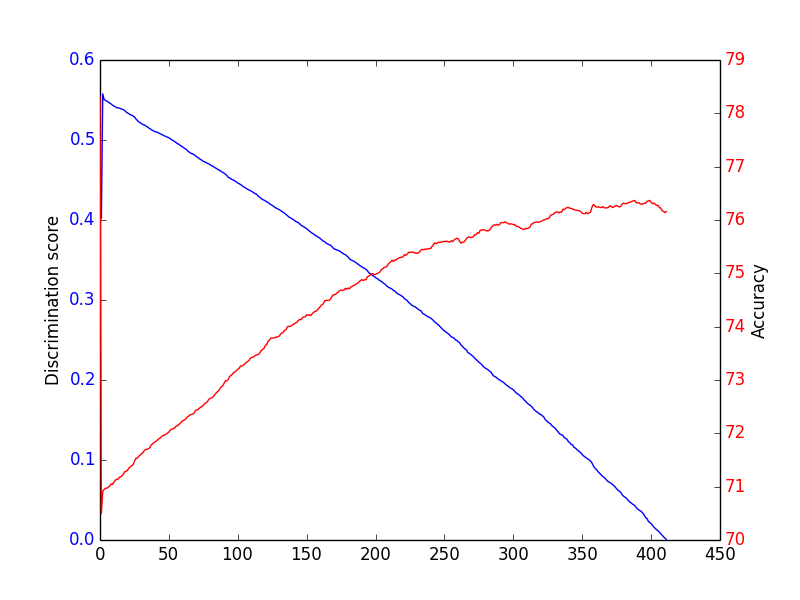
\includegraphics[scale=0.5]{images/modified_optimization.png}
  \caption[optimization]
   {Optimization progression, with Accuracy Vs. Discrimination score on Modified Bayes Model}
\end{figure}


%------------------------------------------------

\begin{thebibliography}{9} 

\bibitem{calders10} \emph{Three naive Bayes approaches for discrimination-free
classification}, Toon Calders et al., 2015.

\bibitem{Zemel13} \emph{Learning Fair Representations}, Richard Zemel et al., 2013

\bibitem{Ruggieri10} \emph{Data Mining for Discrimination Discovery}, Salvatore Ruggeri et al., 2010 

\bibitem{dataset} \emph{UCI Census Income Data Set}, https://archive.ics.uci.edu/ml/datasets/Census+Income

\bibitem{uc_repo} \emph{{UCI} Machine Learning Repository}
M. Lichman, 2013, http://archive.ics.uci.edu/ml , University of California, Irvine, School of Information and Computer Sciences


\end{thebibliography}

\end{document}